\section{Background}

\begin{paraphrase}
 In this section, we present some of design basics (often simplified to aid readability) of FAT file system and NTFS file system, 
which are relevant to what we discuss in the latter part of the paper. 
We highlight what information remains in the file system after a file is deleted, 
which leads to understanding of how metadata-based file-recovery might work. 
Finally, we present the \emph{core features} of NIST standards for such recovery tools.  
\end{paraphrase}

\TODO{Add a few lines about carving}


\subsection{FAT File System}
\begin{paraphrase}
 As in many other file systems, a file in FAT system has metadata in addition to the actual file content. 
The main metadata of a file (say foo.txt) in FAT system is called a \emph{directory entry}, which is of 32 bytes.
The directory entry of a file (say foo.txt) has three main \emph{essential} elements: (a) file name, (b) file size, and 
(c) index of the starting cluster (which holds the actual file content). We can figure 
out the index of other clusters of the file by reading a global table called the FAT table. The FAT table
can determine the chain of clusters which hold the data of a file. In particular, 
for each cluster (say x) of the file system, the FAT table has an entry, and 
if FAT(x) is 0, then that means cluster x is currently unallocated. 
On the other hand, if FAT(x) is y, then that means cluster y is the next cluster after cluster x (as part of the same file).
If FAT(x) is EOF, that indicates cluster x is the last cluster of the file.
   
As an example, the directory entry of foo.txt and the clusters (holding the actual content of foo.txt) 
are illustrated in Figure~\ref{fig:fat1}. The FAT table is also shown, which tells us that foo.txt's data is stored 
in contiguous clusters, starting from cluster 100 and ending at cluster 200.

% \begin{figure}[h]
%     \centering
%     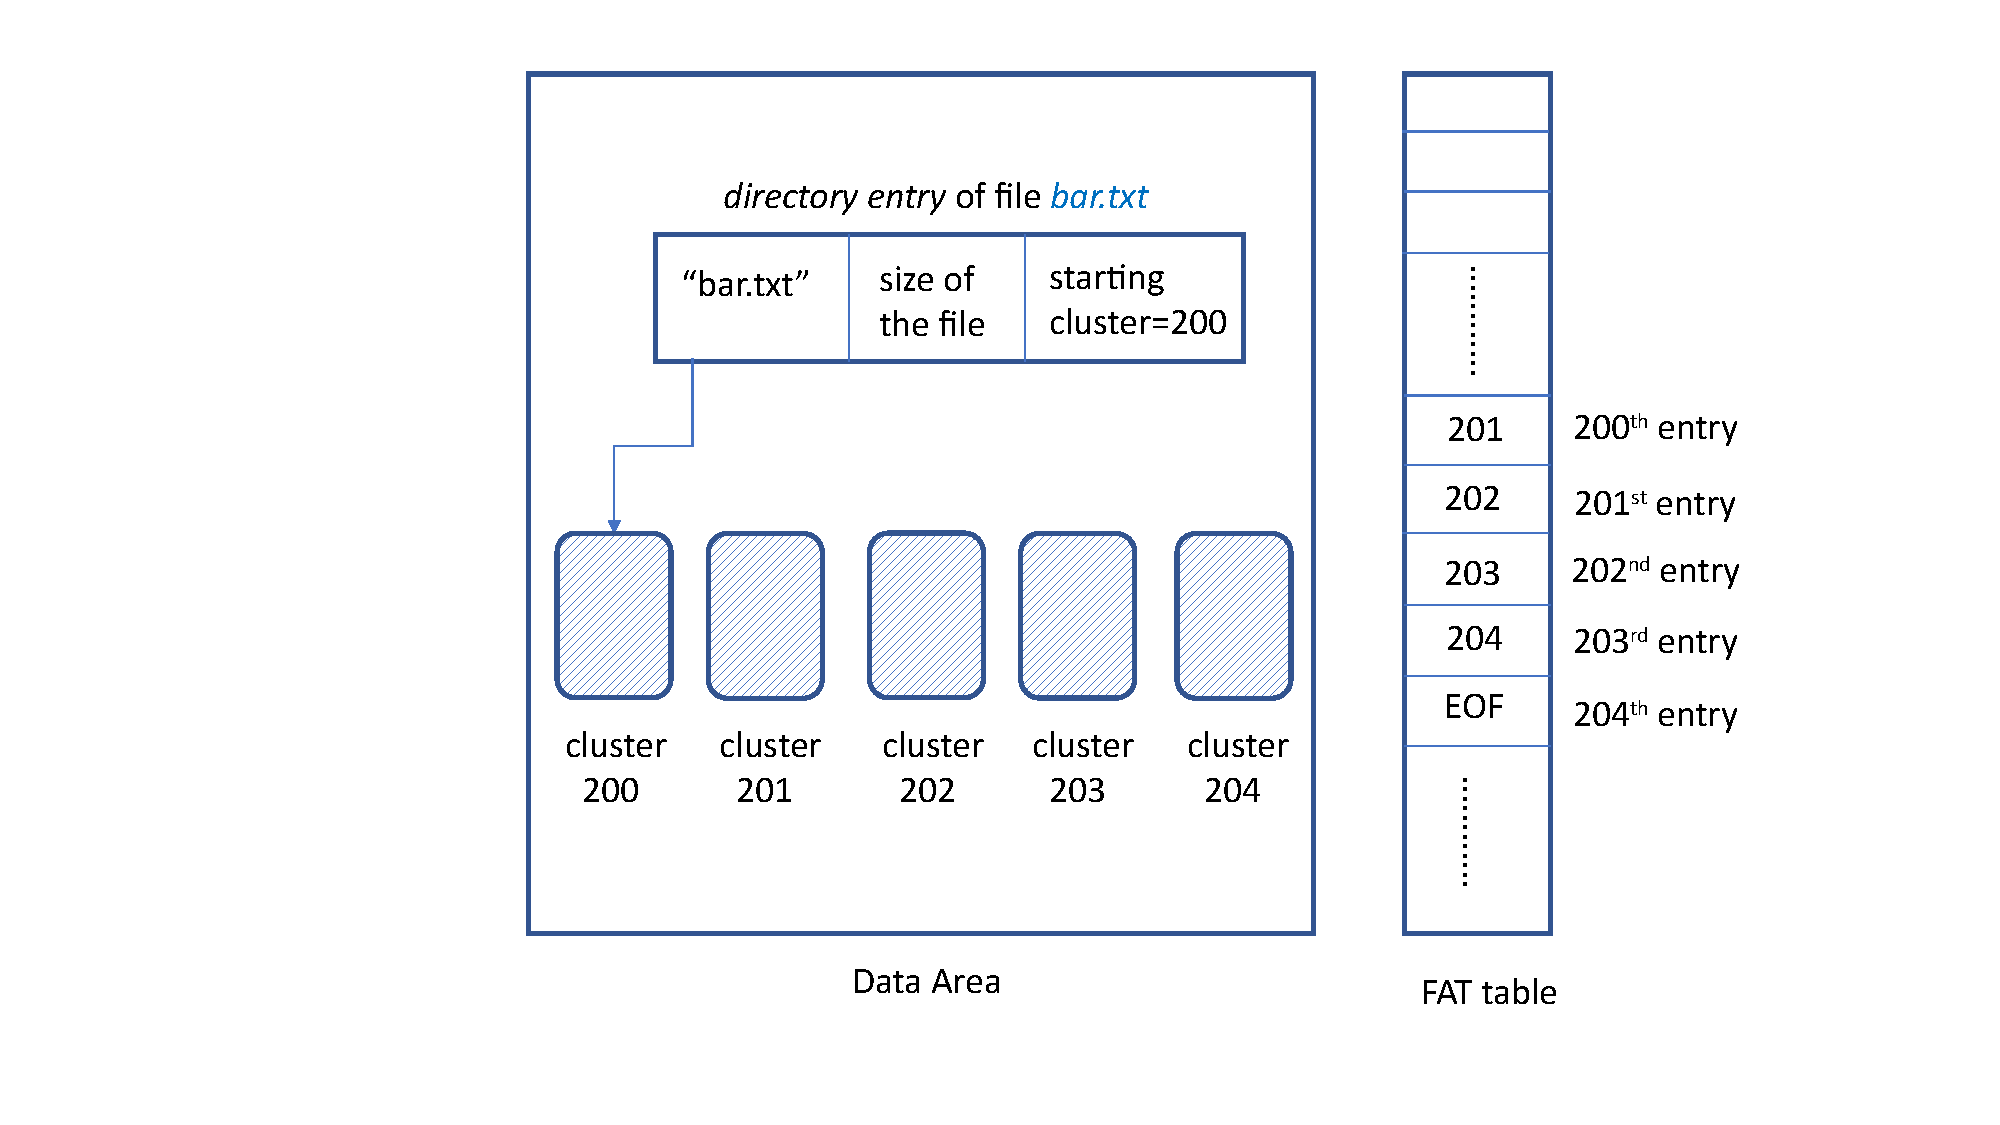
\includegraphics[width=\linewidth]{fig/fat1.pdf}
%     \caption{File foo.txt in a FAT file system. The \emph{directory entry} of this file and the actual file content clusters (shaded) are shown. 
% The FAT table is also shown, which determines the chain of clusters (from cluster 100 to cluster 200) of foo.txt.}
%     \label{fig:fat1}
% \end{figure}


The change in metadata and actual content of foo.txt is illustrated in Figure~\ref{fig:fat2} after the file is deleted.
The first character of the file name (say ``foo.txt") is flagged (``\_oo.txt") to denote that the file is deleted, 
but the remaining part of the directory entry can be still available. In the FAT table, the deleted file's corresponding
entries are \emph{zeroed}, which denotes that those clusters are available to be allocated to a new file (if necessary).
However, the actual content carrying clusters (say cluster 100 to cluster 200)
can still be intact until they are \emph{overwritten} by another file. 
  
% \begin{figure}[h]
%     \centering
%     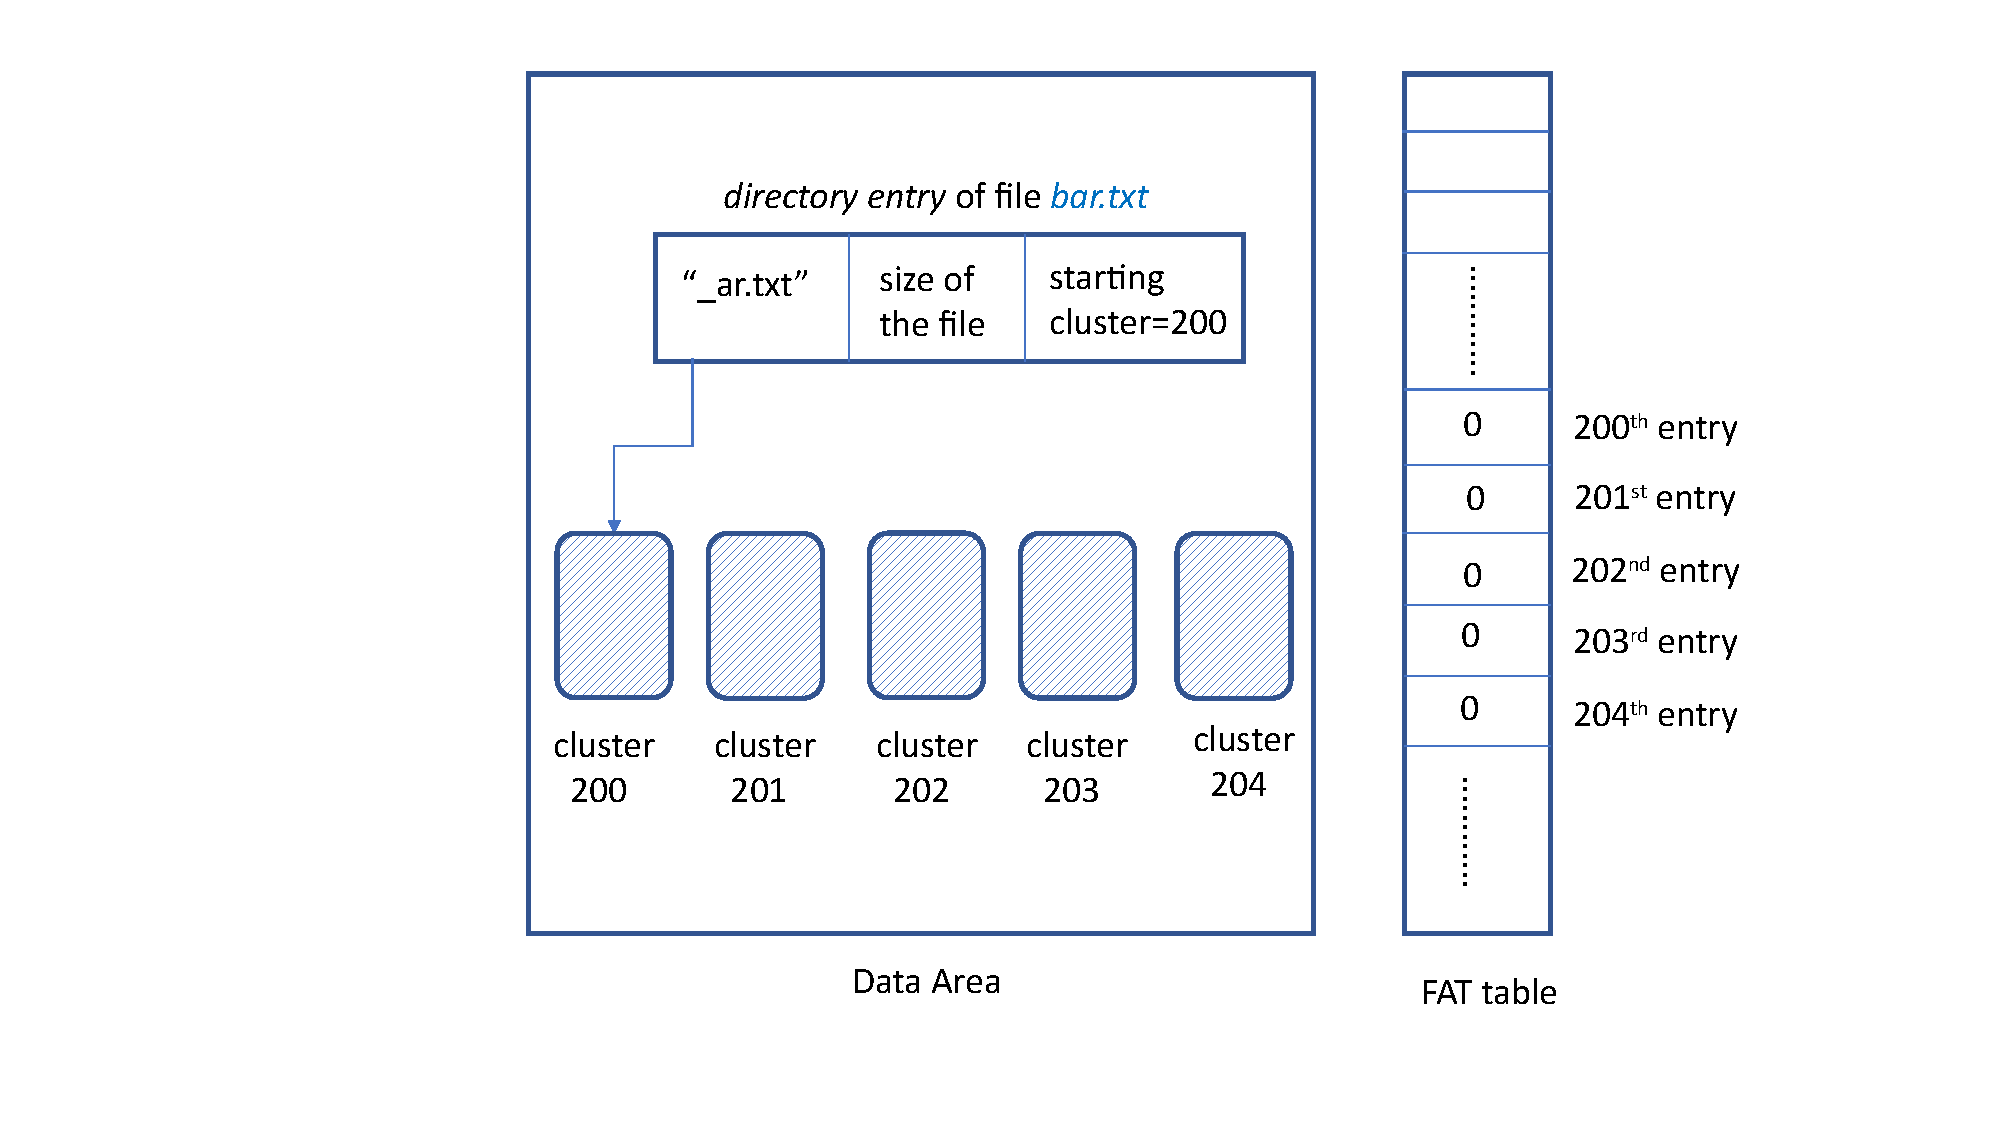
\includegraphics[width=\linewidth]{fig/fat2.pdf}
%     \caption{The metadata and actual content of foo.txt are shown after the file is deleted whereas the corresponding entries (i.e., 100-200) in the FAT table are zeroed.}
%     \label{fig:fat2}
% \end{figure}

Furthermore, it is possible that the content of a file is not stored in contiguous clusters in FAT file system, 
and this phenomenon is called \emph{fragmentation}.
If the original file foo.txt has two fragments, it may look as illustrated in Figure~\ref{fig:fat3} where the file's first fragment is from cluster 100 to cluster 101 and the 
second fragment is from cluster 200 to cluster 298. 

% \begin{figure}[h]
%     \centering
%     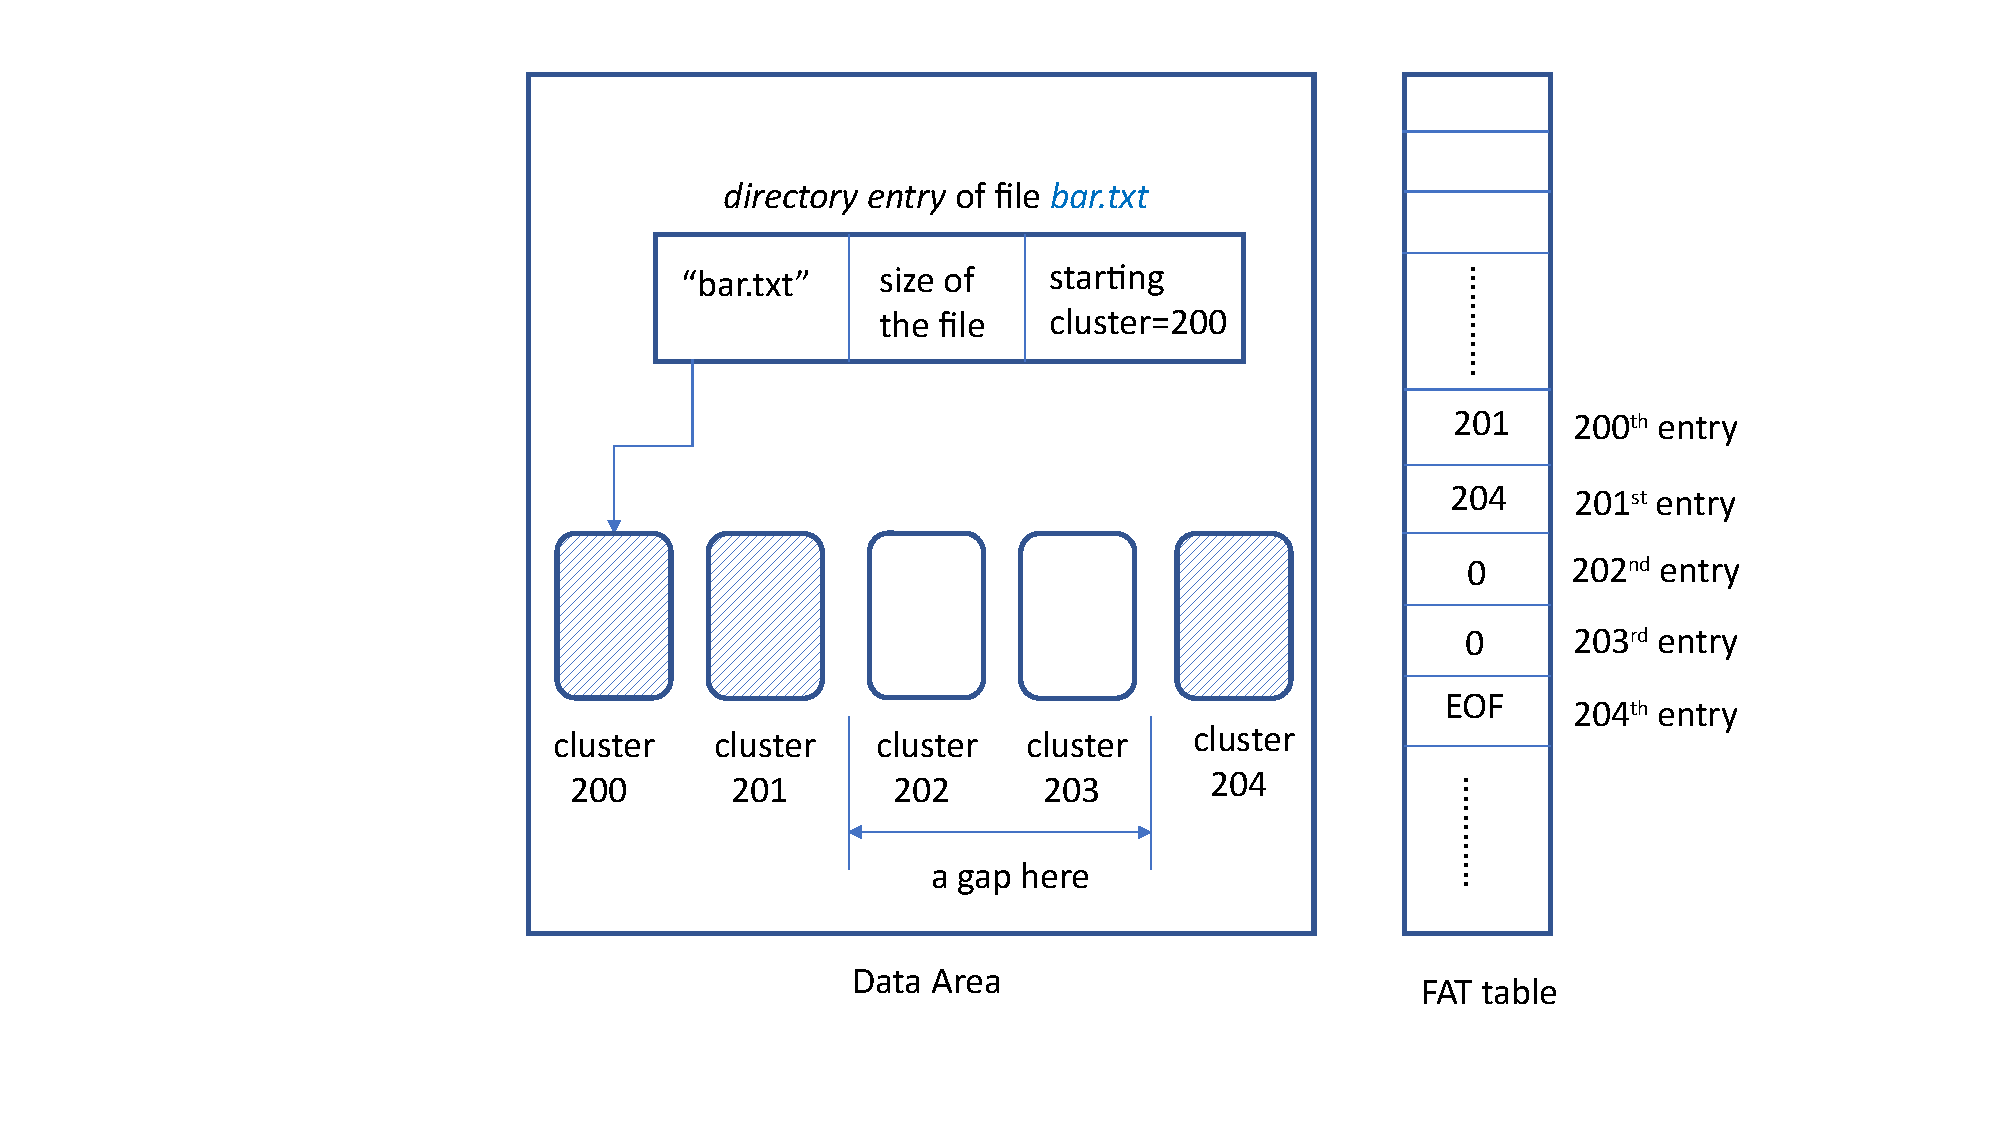
\includegraphics[width=\linewidth]{fig/fat3.pdf}
%     \caption{The layout of metadata and actual content of a file foo.txt is shown whereas the file has two fragments (cluster 100-101 and cluster 200-298) 
% as determined by the FAT table.}
%     \label{fig:fat3}
% \end{figure}
\end{paraphrase}



\subsection{NTFS File System}
\begin{paraphrase}

In an NTFS system, each file has an entry in the Master File Table (MFT) where every entry is typically 1024 bytes. 
If a file is short, then all of its metadata as well as the actual content can sit inside the MFT entry; otherwise, 
the file content can be non-resident (i.e., not in MFT entry) and located in other clusters.
  
As an example, the MFT entry of foo.txt and the actual content carrying clusters are illustrated in Figure~\ref{fig:ntfs}.
The MFT entry indicates that there are two runs of clusters (100-101 and 200-298) which carry the actual file content. 
In this case, the example file has two fragments.

% \begin{figure}[h]
%     \centering
%     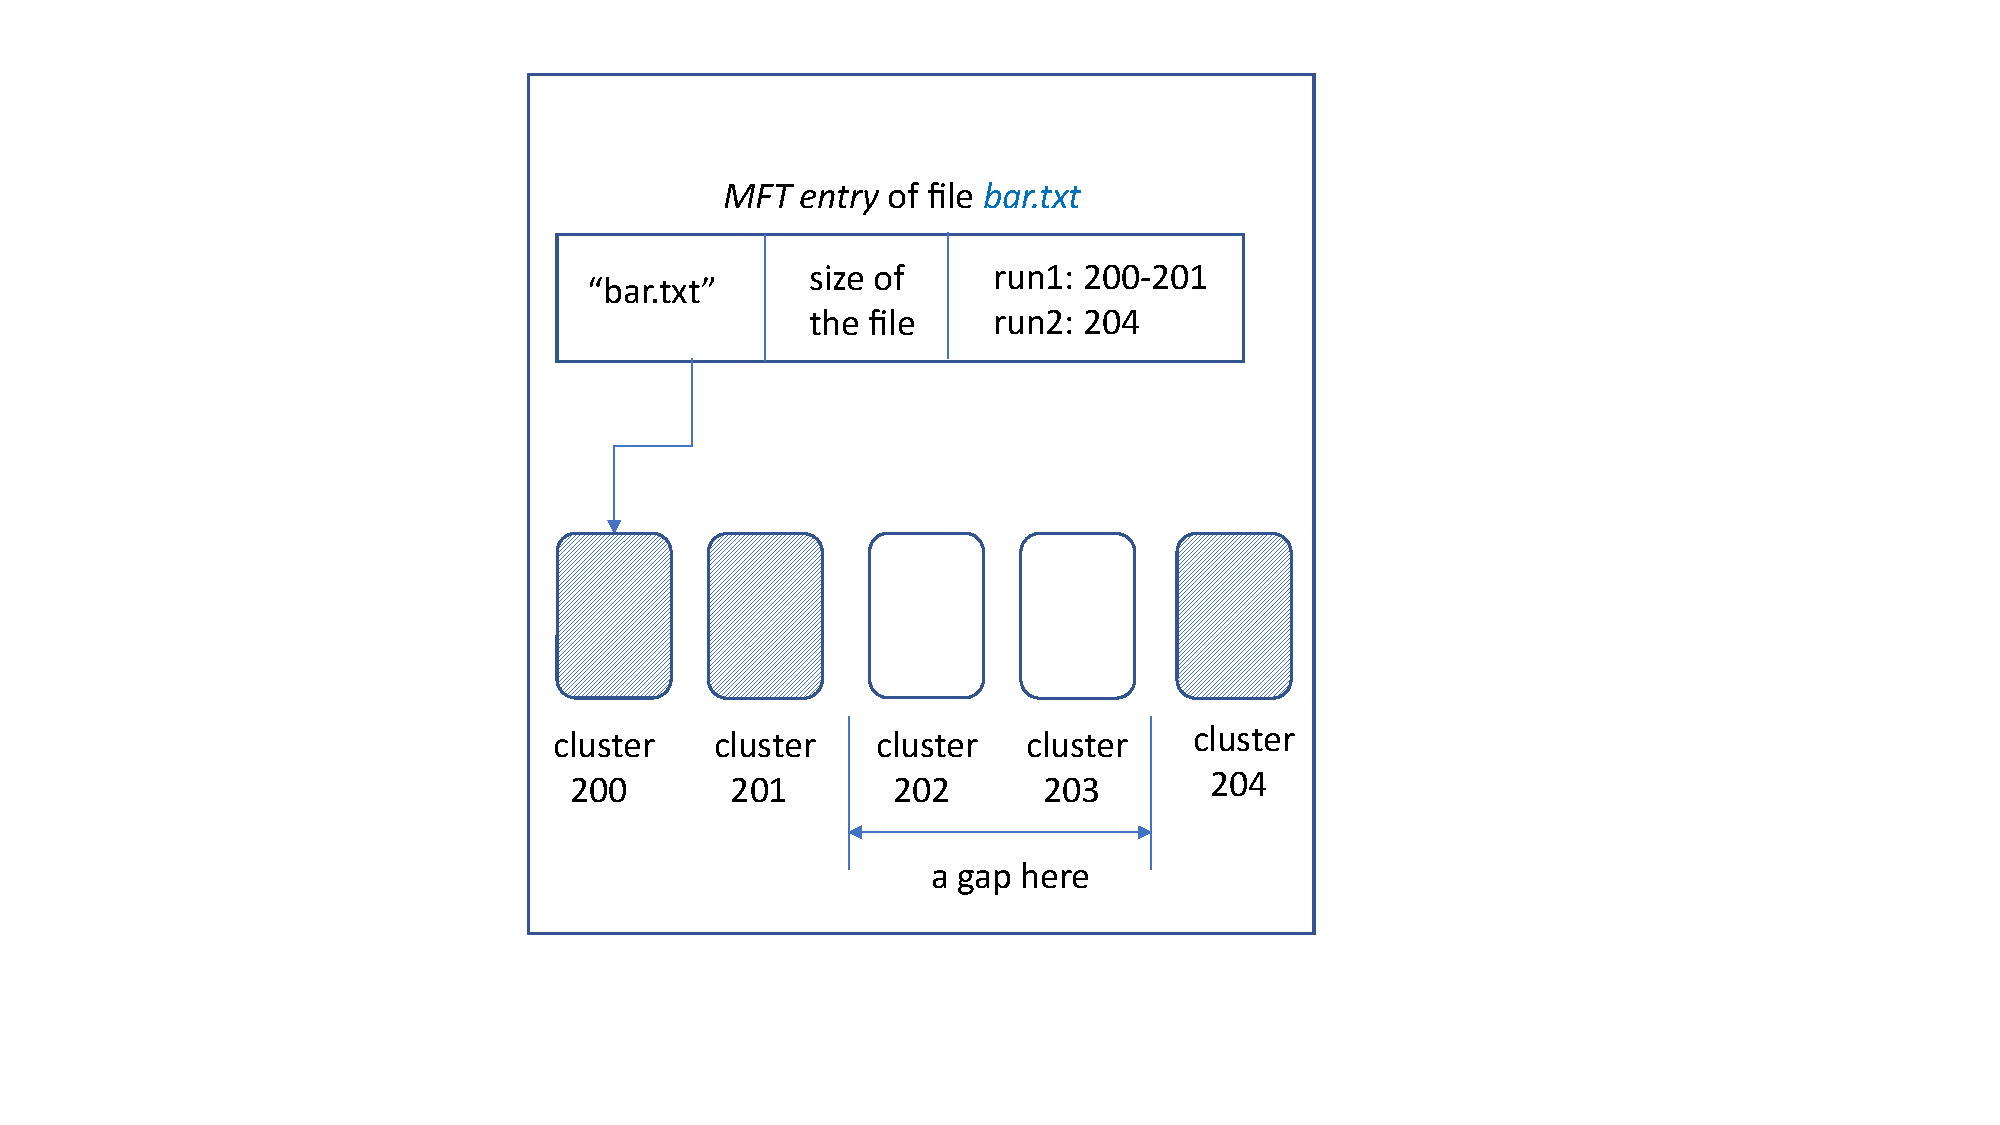
\includegraphics[width=\linewidth]{fig/ntfs.pdf}
%     \caption{To illustrate NTFS file system, the MFT entry of foo.txt and the actual content carrying clusters are shown. 
% This file has two fragments (cluster 100-101 and cluster 200-298).}
%     \label{fig:ntfs}
% \end{figure}
 
\end{paraphrase}

\subsection{Metadata-Based Deleted File Recovery}
\begin{paraphrase}
 The previous discussion implies that in many cases a deleted file's metadata 
(e.g., directory entry in FAT or MFT entry in NTFS) can be still available, 
and it is possible to recover the file content using this metadata. 
This is called metadata-based deleted file recovery.

For instance, in the example of Figure~\ref{fig:fat2},
we can see from the directory entry of foo.txt that 
the deleted file starts in cluster 100 and has a size of 101 clusters;
thus, we can reason that the deleted file content is in cluster 100 to cluster 200.
We can recover the whole file via reading the raw content of these clusters (e.g., by using dd command in Kali Linux). 

Note that in FAT system the \emph{directory entry} of a file only refers to the starting cluster, and it does not carry any information about the file fragments.
That is why in certain situations where the deleted file is fragmented, metadata-based file recovery in FAT system encounters challenges.
On the other hand, if a file is fragmented in NTFS, the corresponding MFT entry does contain information on all the runs (i.e., fragments) of the file
(as shown in Figure~\ref{fig:ntfs}). Consequently, fragmentation does not introduce any extra challenge in file recovery in NTFS.
\end{paraphrase}

\subsection{File Carving}

\TODO{TODO}

\subsection{NIST Guidelines}
\subsubsection{For Metadata-Based DFR}
\begin{paraphrase}
 The NIST guidelines~\cite{meta:dfr:standards} list four \emph{core features} upon which metadata-based DFR tools are to be judged.
Following is the text of each core feature as well as our interpretation of each in the context of this work:

 \paragraph{DFR-CR-01} ``The tool shall identify all deleted File System-Object entries accessible in residual metadata''~\cite{meta:dfr:standards}.
 We consider a tool passing this standard if it identifies to the user each file system metadata entry that is marked as deleted.
 \paragraph{DFR-CR-02} ``The tool shall construct a Recovered Object for each deleted File System-Object entry accessible in residual metadata''~\cite{meta:dfr:standards}.
 We consider a tool passing this standard as long as it outputs a file for each deleted file, even if the output file is empty.
 \paragraph{DFR-CR-03} ``Each Recovered Object shall include all non-allocated data blocks identified in a residual metadata entry''~\cite{meta:dfr:standards}.
 For FAT file systems, we consider a tool passing this standard if it recovers at least the first contiguous segment of unallocated sectors starting 
from the first sector originally allocated to the deleted file. For NTFS file systems, the tool must recover all unallocated sectors originally allocated to the deleted file.
 \paragraph{DFR-CR-04} ``Each Recovered Object shall consist only of data blocks from the Deleted Block Pool''~\cite{meta:dfr:standards}.
 We consider a tool passing this standard if the recovered file consists only of data from the original deleted file, or null data to represent omitted portions.


\end{paraphrase}

\subsubsection{For File Carving} \label{sec:carving_features}

\begin{paraphrase}
 The NIST guidelines~\cite{carving_standards} list five \emph{core features} upon which file carving DFR tools are to be judged.
Following is the text of each core feature as well as our interpretation of each in the context of this work:
\end{paraphrase}

 \paragraph{FC-CR-01} ``The tool shall return one carved file for each supported file header signature from a source file that is present in the search arena''.~\cite{carving_standards}
 
 Each file from the original disk will begin with a header signature specific to its file format. We consider a tool as passing this guideline if it carves a file starting at each of those header signatures.
 In other words, tools that perform well on this core feature have a high ``hit rate.''
 
 \paragraph{FC-CR-02} ``A carved file shall only contain data blocks from the search arena''.~\cite{carving_standards}
 
 In other words, the tool should only work within the drive or partition it is given, and should not try to carve from out-of-bounds.
 
 \paragraph{FC-CR-03} ``All data blocks in a carved file shall originate in a single source file''.~\cite{carving_standards}
 
We consider a tool as passing if each recovered file only contains data from one file on the original disk.
 
 \paragraph{FC-CR-04} ``The file type of a carved file shall match the file type of its contents''.~\cite{carving_standards}
 
 We interpret this to mean that the file extension given to a recovered file must accurately describe the format of the file data. We exclude false positives from this evaluation because their data is highly unlikely to be of any file format. So, we only consider files which were carved starting from a valid header signature.
 
 \paragraph{FC-CR-05} ``The tool shall return carved files in a state that conforms to a valid file of the carved file type''.~\cite{carving_standards}
 
 We consider a tool as passing if each recovered file can be parsed without error by some application software.
 We use the ImageMagick tool suite to evaluate this.
